\section{Modelo de Despliegue}

\begin{figure}[h]

  \centering
  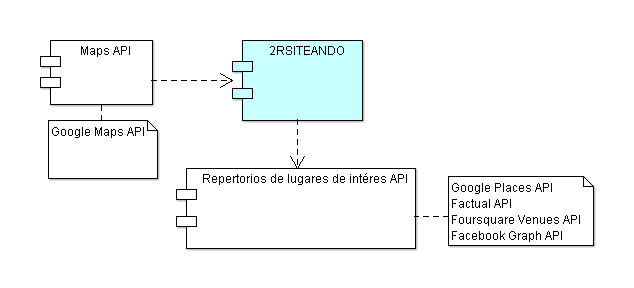
\includegraphics[width=18cm,height=6cm]{Imagenes/Despliegue/modelo_despliegue_exterior.png}
  \caption{Diagrama de despliegue exterior}  

\end{figure}

El sistema va a interactuar con otros dos tipos de sistemas principales.
\newline

El primero es un sistema de mapa interactivo, que ofrece una API permitiendo trazar rutas y ubicar puntos. Por esto se utilizar\'a Google Maps API, que tiene una muy buena capacidad de integraci\'on con Android y permite su el uso desde un servidor.
\newline

El segundo es un sistema de enumeraci\'on y de descubrimiento de lugares de inter\'es, que ofrece una API permitiendo consultar una lista de lugares por coordinadas geogr\'aficos y otros criterios. Se utilizara los servicios de Google Places API, Factual API, Foursquare Venues API o Facebook Graph API. 
Es recomendable utilizar dos o m\'as de dichos servicios de manera simult\'anea.


\begin{figure}[h]

  \centering
  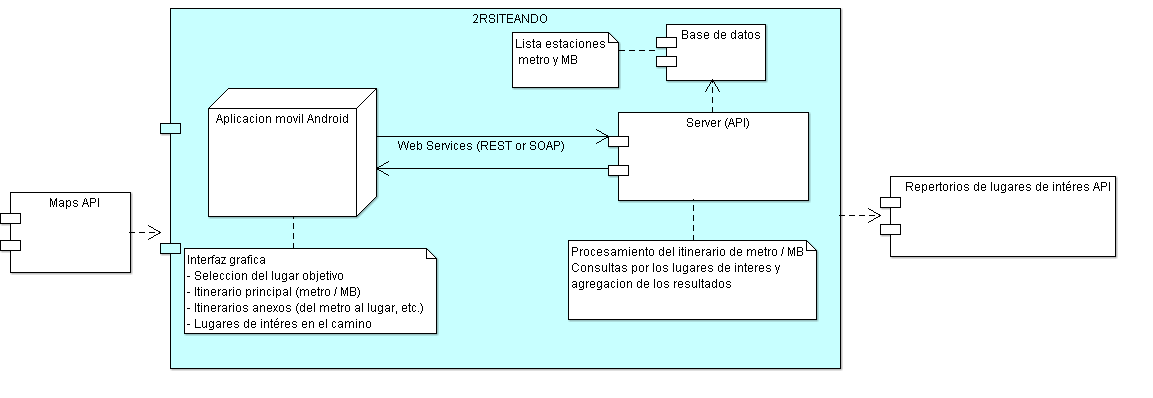
\includegraphics[width=18cm,height=6cm]{Imagenes/Despliegue/modelo_despliegue_interior.png}
  \caption{Diagrama de despliegue interior}  

\end{figure}

El diagrama de despliegue interior da a conocer la integraci\'on de los dos servicios exteriores,  previamente presentados. Es importante destacar la comunicaci\'on entre la aplicaci\'on Android y el servidor y sus responsabilidades.
\newline

Para comunicar la aplicaci\'on Android y el servidor, se utilizar\'an servicios web, con probabilidad de tipo REST.
\newline

El servidor ser\'a encargado de calcular el itinerario global, conociendo la ubicaci\'on del usuario y su(s) destinos. El usuario determinar\'a que transportes p\'ublico utilizar\'a (metro o metrobus) y cual partes del itinerario van a ser peatonales (recorte de la ruta en fracciones). 
Entonces, hay una capa de abstracci\'on por la manera de calcular la ruta para la aplicaci\'on Android, que solamente se encargue mostrarla, sin conocimiento del algoritmo utilizado. Para calcular esta ruta, el servidor va a utilizar una base de datos de los estaciones y aplicar un algoritmo de la teor\'ia de los grafos.
\newline

Adem\'as, el servidor debe ser capaz de proporcionar a la aplicaci\'on Android los lugares de inter\'es cercanos al lugar inicial de interes. De esta manera, la aplicaci\'on Android no necesita ser conciente de quien proporciona los lugares de inter\'es, que sea una o diferentes API exteriores o que sea una base de datos del servidor en s\'i mismo (otra capa de abstracci\'on).
